% This must be in the first 5 lines to tell arXiv to use pdfLaTeX, which is strongly recommended.
\pdfoutput=1
% In particular, the hyperref package requires pdfLaTeX in order to break URLs across lines.

\documentclass[11pt]{article}

% Remove the "review" option to generate the final version.
\usepackage[]{acl}

% Standard package includes
\usepackage{natbib}
\usepackage{lastpage}
\usepackage{fancyhdr}
\usepackage{times}
\usepackage{latexsym}
\usepackage{float}
\usepackage{graphicx}

% For proper rendering and hyphenation of words containing Latin characters (including in bib files)
\usepackage[T1]{fontenc}
% For Vietnamese characters
% \usepackage[T5]{fontenc}
% See https://www.latex-project.org/help/documentation/encguide.pdf for other character sets

% This assumes your files are encoded as UTF8
\usepackage[utf8]{inputenc}

% This is not strictly necessary, and may be commented out,
% but it will improve the layout of the manuscript,
% and will typically save some space.
\usepackage{microtype}

\pagestyle{fancy}
\fancyhead{}
\renewcommand{\headrulewidth}{0pt}
\fancyfoot[C]{Page \thepage \hspace{1pt} of \pageref{LastPage}}

% If the title and author information does not fit in the area allocated, uncomment the following
%
%\setlength\titlebox{<dim>}
%
% and set <dim> to something 5cm or larger.

\title{Detecting AI-Generated Images using ResNet}

\author{Ziyang Zeng \and Zhehu Yuan \and Yifan Jin \\
  Dept. of Computer Science \\
  New York University \\
  251 Mercer Street, New York, NY \\
  \texttt{zz2960@nyu.edu, zy2262@nyu.edu, yj2063@nyu.edu}}

\begin{document}
\maketitle
\begin{abstract}
  Abstract goes here.
\end{abstract}

\section{Introduction}

Introduction goes here.


\section{Related Work}

Related work goes here.

\section{Datasets}

In order to train a classifier that can distinguish between real and generated images, we need a labeled dataset that consists  of both real and generated images for supervised learning. Datasets of this kind is not common, and we'd like to experiment on the latest state-of-the-art image generation AI models, such as DALL·E 2 and Stable Diffusion. We started with real photos from existing public datasets as our raw datasets. Then, we use Diffusers-based image-to-image model to generate images from real photos. This way, we can get a labeled dataset that consists of both real and generated images.

\subsection{Raw Datasets}

The original real-world photos we experimented with are from public datasets: Indoor Scene Recognition Database and Weather Image Recognition Dataset. Additionally, we want to test how well our model performs on non-photo art work. A dataset that consists of pages of comic art (the Comic Books Images Dataset) is also used in our experiments.

\subsubsection{Indoor Scene Recognition Database}

Originally targeting at indoor scene recognition tasks, the Indoor Scene Recognition Database is a collection of 67 indoor categories (e.g. airport, living room, restaurant...) and at least 100 images per category. There are 15,620 images in the dataset in total. Figure \ref{fig:paper_indoor_dataset} shows some examples of the dataset.

\begin{figure}[h]
  \centering
  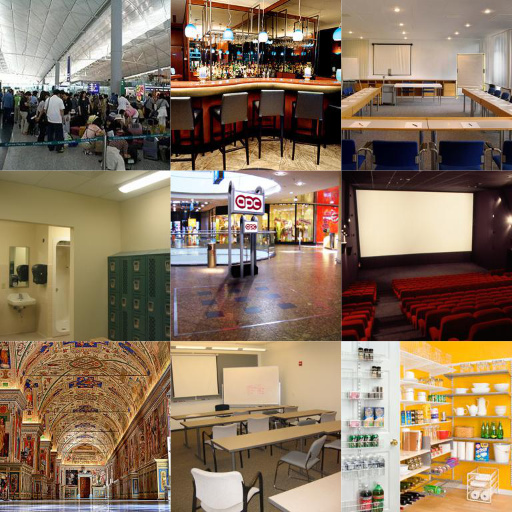
\includegraphics[width=140]{./assets/paper_indoor_dataset.jpg}
  \caption{Indoor Scene Recognition Database Examples}
  \label{fig:paper_indoor_dataset}
\end{figure}

This dataset is the biggest among the three datasets we used and serves as our main dataset. We use the AI-generated variations from these images and the images themselves to train our classifier.

\subsubsection{Weather Image Recognition Dataset}

The Weather Image Recognition Dataset contains labeled 6862 images of different types of weather, its catogories including dew, fog, frost, glaze, etc. This dataset is used in our experiment to evaluate our model's generalization ability and performance on other kinds of photos than indoors.

\begin{figure}[h]
  \centering
  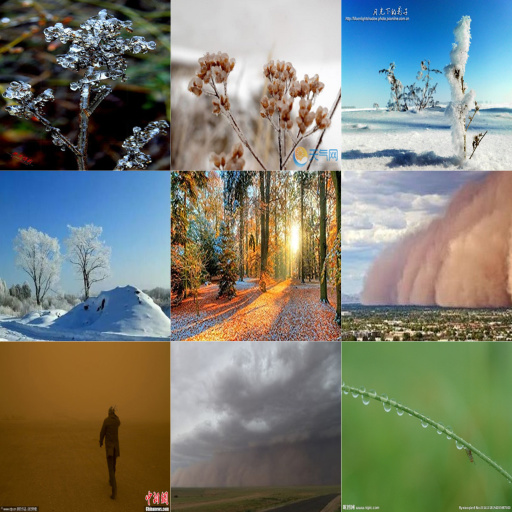
\includegraphics[width=140]{./assets/paper_weather_dataset.jpg}
  \caption{Weather Image Recognition Dataset Examples}
  \label{fig:paper_weather_dataset}
\end{figure}

\subsubsection{Comic Books Images Dataset}

\subsection{Diffusers}

\subsubsection{CLIP guidance}

\subsubsection{Stable Diffusion}


Some examples of the real-world pictures are:

\begin{figure}[htbp]
\centering
\subfigure{
\begin{minipage}[t]{0.3\linewidth}
\centering
\includegraphics[width=1.2in]{paper/assets/original_airport_inside_airport_inside_0001.jpg}
\caption{airport}
\end{minipage}%
}%
\ \  \ \  \ \  \ \
\subfigure {
\begin{minipage}[t]{0.3\linewidth}
\centering
\includegraphics[width=1.2in]{paper/assets/original_winecellar_wineCellar01.jpg}
\caption{wineCellar}
\end{minipage}%
}%
\end{figure}


The corresponding AI-generated pictures are:


\begin{figure}[htbp]
\centering
\subfigure{
\begin{minipage}[t]{0.3\linewidth}
\centering
\includegraphics[width=1.2in]{./assets/ai_airport_inside_airport_inside_0001.jpg}
\caption{airport}
\end{minipage}%
}%
\ \  \ \  \ \  \ \
\subfigure {
\begin{minipage}[t]{0.3\linewidth}
\centering
\includegraphics[width=1.2in]{./assets/ai_winecellar_wineCellar01.jpg}
\caption{wineCellar}
\end{minipage}%
}%
\end{figure}



\subsubsection{DALL·E 2}

\subsubsection{Image Variation Generation}

\section{Classifier}

Classifier goes here.

\section{Experiments}



\subsection{Experiment Settings}

\subsubsection{Training}

The whole dataset includes 15620 real-world indoor pictures together with 15620 AI-generated pictures. Each real-world picture generates one AI pictures using the stable diffusion model.

Around 80\% pictures for each type are used for training.


In terms of the model, we use the resnet34 intergrated inside the fastai.

\subsubsection{Validation}

We picked around 20\% pictures of the above indoor pictures for each type as the validation dataset. The validation data is not used in the training process.

\subsubsection{Testing}

The testing dataset includes several types of pictures:

(1) 6738 real-world weather pictures together with 6738 AI-generated pictures. Each real-world picture generates one AI pictures using the stable diffusion model.

(2) Comic pictures

(3) Dalle dataset where AI pictures are generated by dalle model, not stable diffusion model.

\subsection{Evaluation Metrics}

To evaluate the performance of the model, we used accuracy, precision, recall and F1-score as evaluation metrics. Below are the formulas for calculating the accuracy, precision, recall and F1-score. Here we assume the AI-generated pictures as positive labels while original pictures as negative labels. Thus, TP is the number of AI pictures being correctly predicted as AI pictures, FP is the number of original pictures being wrongly predicted as AI pictures. Similarly, TN is the number of original pictures being correctly predicted as original pictures, FN is the number of AI pictures being wrongly predicted as original pictures.

\[
Accuarcy = \frac{TP+TN}{TP+FP+TN+FN}
\]
\[
Precision = \frac{TP}{TP+FP}
\]
\[
Recall = \frac{TP}{TP+FN}
\]
\[
F1 = \frac{2 \times Precision \times Recall}{Precision + Recall}
\]


\section{Experiment Results}

Experiment results go here.

\begin{figure}[htbp]
\centering
\subfigure{
\begin{minipage}[t]{\linewidth}
\centering
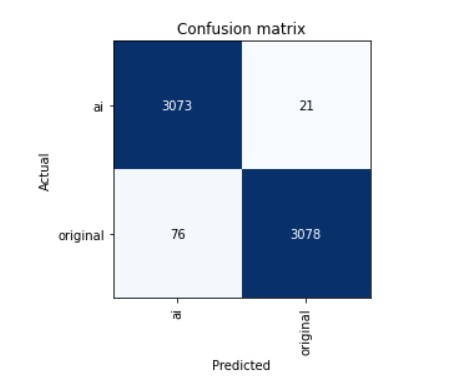
\includegraphics[width=4in]{paper/training_confusion_matrix.jpg}
\caption{Validation Confusion Matrix}
\end{minipage}%
}%
\end{figure}

\section{Conclusion}

Conclusion goes here.

\section{Discussion and Future Work}

Discussion and future work go here.

% \printbibliography
\bibliographystyle{plain}
\bibliography{refs}

\end{document}
